% Previous horizontal figure preserved for review:
% % Native TikZ source for the lookup-work panel.
% % Values are from the D_pinned_5pct rows in:
% %   vcomp/experiments/results/paper_figure4_uniform_read_cache_5m_single.tsv
% % Each row is one 300-second, 48-thread uniform YCSB-C run over a database
% % built from a 1,000 GiB logical input. Bars show Bloom-filter checks per
% % lookup; diamonds show Bloom-positive candidate SSTs per lookup.
% % The x positions below use a true logarithmic mapping over [0.45, 40000].
% \begingroup
% \definecolor{altBaseline}{HTML}{5B5B5B}
% \definecolor{altFlush}{HTML}{E69F00}
% \definecolor{altLast}{HTML}{F0A83B}
% \definecolor{altFillseq}{HTML}{009E73}
% \definecolor{altFillseqOw}{HTML}{4AAE91}
% \definecolor{altFtwo}{HTML}{0072B2}
% \begin{tikzpicture}[
%     x=1cm,
%     y=1cm,
%     font=\small,
%     axis/.style={draw=black!80, line width=0.50pt},
%     grid/.style={draw=black!16, line width=0.40pt},
%     baselinebar/.style={draw=black!85, fill=altBaseline, line width=0.45pt},
%     flushbar/.style={draw=black!85, fill=altFlush, line width=0.45pt},
%     lastbar/.style={draw=black!85, fill=altLast, line width=0.45pt},
%     fillseqbar/.style={draw=black!85, fill=altFillseq, line width=0.45pt},
%     fillseqowbar/.style={draw=black!85, fill=altFillseqOw, line width=0.45pt},
%     f2loadbar/.style={draw=black!85, fill=altFtwo, line width=0.45pt},
%     positive/.style={draw=black, fill=white, line width=0.55pt}
% ]
% \path[use as bounding box] (-0.03,-0.43) rectangle (5.82,5.12);
% 
% % Logarithmic x-axis. Plot origin 1.80 corresponds to 0.45 SSTs/lookup;
% % plot end 5.40 corresponds to 40,000 SSTs/lookup. The constants below are
% % -ln(0.45) and ln(40000)-ln(0.45), written explicitly because TeX's
% % fixed-point arithmetic cannot first represent the literal 40000.
% \foreach \tick/\ticklabel in {1/1,10/10,100/100,1000/{1K},10000/{10K}} {
%     \pgfmathsetmacro{\tickx}{
%         1.80 + 3.60*(ln(\tick)+0.7985076962)/11.3951424293}
%     \draw[grid] (\tickx,0.35) -- (\tickx,5.02);
%     \draw[axis] (\tickx,0.29) -- (\tickx,0.35);
%     \node[anchor=north, font=\scriptsize] at (\tickx,0.24) {\ticklabel};
% }
% \draw[axis] (1.80,0.35) -- (5.40,0.35);
% \draw[axis] (1.80,0.35) -- (1.80,5.02);
% 
% % y / system / filter checks / Bloom-positive candidates / shown checks /
% % bar style. The full-precision promoted values determine the geometry.
% \foreach \y/\system/\checks/\positives/\shown/\barstyle in {
%     4.65/{Baseline}/3.618606635/0.660687518/3.62/baselinebar,
%     3.87/{Flush-only}/10253.243996632/99.757193700/{10.3K}/flushbar,
%     3.09/{Last-comp}/0.999994131/0.635706963/1.00/lastbar,
%     2.31/{Fillseq}/1.000000000/1.000000000/1.00/fillseqbar,
%     1.53/{Fillseq+OW}/3.387641458/1.022472636/3.39/fillseqowbar,
%     0.75/{F2Load}/3.570955689/0.645238291/3.57/f2loadbar%
% } {
%     \pgfmathsetmacro{\barend}{
%         1.80 + 3.60*(ln(\checks)+0.7985076962)/11.3951424293}
%     \pgfmathsetmacro{\positivex}{
%         1.80 + 3.60*(ln(\positives)+0.7985076962)/11.3951424293}
%     \draw[\barstyle] (1.80,\y-0.20) rectangle (\barend,\y+0.20);
%     \node[anchor=east, font=\scriptsize] at (1.67,\y) {\system};
%     % Four explicit points avoid requiring TikZ's shapes.geometric library.
%     \draw[positive]
%         (\positivex,\y+0.105) -- (\positivex+0.105,\y) --
%         (\positivex,\y-0.105) -- (\positivex-0.105,\y) -- cycle;
%     \node[anchor=west, font=\scriptsize] at (\barend+0.10,\y) {\shown};
% }
% 
% % Legend occupies unused space to the right of the two lowest bars.
% \draw[draw=black!85, fill=black!35, line width=0.45pt]
%     (3.28,1.34) rectangle (3.57,1.55);
% \node[anchor=west, font=\scriptsize] at (3.73,1.445) {Filter checks};
% \draw[positive]
%     (3.43,1.03) -- (3.535,0.925) -- (3.43,0.82) -- (3.325,0.925) -- cycle;
% \node[anchor=west, font=\scriptsize] at (3.73,0.925) {Bloom positive};
% 
% \node[anchor=north, font=\small] at (3.60,-0.04) {SSTs / lookup (log)};
% \end{tikzpicture}
% \endgroup

% Previous plotted version preserved for review:
% % Loading: vcomp/experiments/results/paper_figure4_loading_time_1tb_single.tsv
% % Reads: vcomp/experiments/results/paper_figure4_uniform_read_cache_5m_single.tsv
% % One run per cell; all measured values are unchanged by this layout revision.
% \begingroup
% \definecolor{vb0}{HTML}{5B5B5B}
% \definecolor{vb1}{HTML}{E69F00}
% \definecolor{vb2}{HTML}{F0A83B}
% \definecolor{vb3}{HTML}{009E73}
% \definecolor{vb4}{HTML}{4AAE91}
% \definecolor{vb5}{HTML}{0072B2}
% \begin{tikzpicture}[x=1cm,y=1cm,font=\small,
% axis/.style={draw=black!80,line width=0.5pt},
% grid/.style={draw=black!16,line width=0.4pt}]
% \path[use as bounding box] (0,0) rectangle (5.200,5.650);
% \draw[grid] (0.85,1.6312) -- (5.1300,1.6312);
% \draw[axis] (0.79,1.6312) -- (0.85,1.6312);
% \node[font=\fontsize{7}{8}\selectfont,anchor=east] at (0.7300,1.6312) {1};
% \draw[grid] (0.85,2.2981) -- (5.1300,2.2981);
% \draw[axis] (0.79,2.2981) -- (0.85,2.2981);
% \node[font=\fontsize{7}{8}\selectfont,anchor=east] at (0.7300,2.2981) {10};
% \draw[grid] (0.85,2.9649) -- (5.1300,2.9649);
% \draw[axis] (0.79,2.9649) -- (0.85,2.9649);
% \node[font=\fontsize{7}{8}\selectfont,anchor=east] at (0.7300,2.9649) {100};
% \draw[grid] (0.85,3.6317) -- (5.1300,3.6317);
% \draw[axis] (0.79,3.6317) -- (0.85,3.6317);
% \node[font=\fontsize{7}{8}\selectfont,anchor=east] at (0.7300,3.6317) {1K};
% \draw[grid] (0.85,4.2985) -- (5.1300,4.2985);
% \draw[axis] (0.79,4.2985) -- (0.85,4.2985);
% \node[font=\fontsize{7}{8}\selectfont,anchor=east] at (0.7300,4.2985) {10K};
% \draw[axis] (0.85,1.4000) -- (5.1300,1.4000);
% \draw[axis] (0.85,1.4000) -- (0.85,4.7000);
% \node[font=\fontsize{7}{8}\selectfont,rotate=90,anchor=south] at (0.1000,3.0500) {SSTs / lookup (log)};
% % baseline: checks=3.618606635, positives=0.660687518
% \draw[draw=black!80,line width=0.4pt,fill=vb0] (1.01000,1.40000) rectangle (1.45000,2.00369);
% \draw[draw=black,fill=white,line width=0.55pt] (1.2300,1.6012) -- (1.3200,1.5112) -- (1.2300,1.4212) -- (1.1400,1.5112) -- cycle;
% \node[font=\fontsize{7}{8}\selectfont,anchor=south] at (1.2300,2.0737) {3.62};
% \node[font=\fontsize{7}{8}\selectfont,rotate=55,anchor=north east] at (1.2300,1.3000) {Baseline};
% % flush_only: checks=10253.243996632, positives=99.757193700
% \draw[draw=black!80,line width=0.4pt,fill=vb1] (1.71000,1.40000) rectangle (2.15000,4.30578);
% \draw[draw=black,fill=white,line width=0.55pt] (1.9300,3.0542) -- (2.0200,2.9642) -- (1.9300,2.8742) -- (1.8400,2.9642) -- cycle;
% \node[font=\fontsize{7}{8}\selectfont,anchor=south] at (1.9300,4.3758) {10.3K};
% \node[font=\fontsize{7}{8}\selectfont,rotate=55,anchor=north east] at (1.9300,1.3000) {Flush-only};
% % last_comp: checks=0.999994131, positives=0.635706963
% \draw[draw=black!80,line width=0.4pt,fill=vb2] (2.41000,1.40000) rectangle (2.85000,1.63124);
% \draw[draw=black,fill=white,line width=0.55pt] (2.6300,1.5901) -- (2.7200,1.5001) -- (2.6300,1.4101) -- (2.5400,1.5001) -- cycle;
% \node[font=\fontsize{7}{8}\selectfont,anchor=south] at (2.6300,1.7012) {1.00};
% \node[font=\fontsize{7}{8}\selectfont,rotate=55,anchor=north east] at (2.6300,1.3000) {Last-comp};
% % fillseq: checks=1.000000000, positives=1.000000000
% \draw[draw=black!80,line width=0.4pt,fill=vb3] (3.11000,1.40000) rectangle (3.55000,1.63125);
% \draw[draw=black,fill=white,line width=0.55pt] (3.3300,1.7212) -- (3.4200,1.6312) -- (3.3300,1.5412) -- (3.2400,1.6312) -- cycle;
% \node[font=\fontsize{7}{8}\selectfont,anchor=south] at (3.3300,1.7012) {1.00};
% \node[font=\fontsize{7}{8}\selectfont,rotate=55,anchor=north east] at (3.3300,1.3000) {Fillseq};
% % fillseq_ow: checks=3.387641458, positives=1.022472636
% \draw[draw=black!80,line width=0.4pt,fill=vb4] (3.81000,1.40000) rectangle (4.25000,1.98459);
% \draw[draw=black,fill=white,line width=0.55pt] (4.0300,1.7277) -- (4.1200,1.6377) -- (4.0300,1.5477) -- (3.9400,1.6377) -- cycle;
% \node[font=\fontsize{7}{8}\selectfont,anchor=south] at (4.0300,2.0546) {3.39};
% \node[font=\fontsize{7}{8}\selectfont,rotate=55,anchor=north east] at (4.0300,1.3000) {Fillseq+OW};
% % f2load: checks=3.570955689, positives=0.645238291
% \draw[draw=black!80,line width=0.4pt,fill=vb5] (4.51000,1.40000) rectangle (4.95000,1.99985);
% \draw[draw=black,fill=white,line width=0.55pt] (4.7300,1.5944) -- (4.8200,1.5044) -- (4.7300,1.4144) -- (4.6400,1.5044) -- cycle;
% \node[font=\fontsize{7}{8}\selectfont,anchor=south] at (4.7300,2.0699) {3.57};
% \node[font=\fontsize{7}{8}\selectfont,rotate=55,anchor=north east] at (4.7300,1.3000) {F2Load};
% \draw[draw=black,fill=black!35] (1.40,5.30) rectangle (1.66,5.46);
% \node[font=\fontsize{7}{8}\selectfont,anchor=west] at (1.7800,5.3800) {Filter checks};
% \draw[draw=black,fill=white] (1.53,5.17) -- (1.62,5.08) -- (1.53,4.99) -- (1.44,5.08) -- cycle;
% \node[font=\fontsize{7}{8}\selectfont,anchor=west] at (1.7800,5.0800) {Bloom positive};
% \end{tikzpicture}
% \endgroup

% Previous plotted version preserved for review:
% % Loading: vcomp/experiments/results/paper_figure4_loading_time_1tb_single.tsv
% % Reads: vcomp/experiments/results/paper_figure4_uniform_read_cache_5m_single.tsv
% % One run per cell; all measured values are unchanged by this layout revision.
% \begingroup
% \definecolor{vb0}{HTML}{5B5B5B}
% \definecolor{vb1}{HTML}{E69F00}
% \definecolor{vb2}{HTML}{F0A83B}
% \definecolor{vb3}{HTML}{009E73}
% \definecolor{vb4}{HTML}{4AAE91}
% \definecolor{vb5}{HTML}{0072B2}
% \begin{tikzpicture}[x=1cm,y=1cm,font=\small,
% axis/.style={draw=black!80,line width=0.5pt},
% grid/.style={draw=black!16,line width=0.4pt}]
% \path[use as bounding box] (0,0) rectangle (6.200,5.650);
% \draw[grid] (0.85,1.4000) -- (5.1300,1.4000);
% \draw[axis] (0.79,1.4000) -- (0.85,1.4000);
% \node[font=\fontsize{7}{8}\selectfont,anchor=east] at (0.7300,1.4000) {0};
% \draw[grid] (0.85,2.0600) -- (5.1300,2.0600);
% \draw[axis] (0.79,2.0600) -- (0.85,2.0600);
% \node[font=\fontsize{7}{8}\selectfont,anchor=east] at (0.7300,2.0600) {1};
% \draw[grid] (0.85,2.7200) -- (5.1300,2.7200);
% \draw[axis] (0.79,2.7200) -- (0.85,2.7200);
% \node[font=\fontsize{7}{8}\selectfont,anchor=east] at (0.7300,2.7200) {2};
% \draw[grid] (0.85,3.3800) -- (5.1300,3.3800);
% \draw[axis] (0.79,3.3800) -- (0.85,3.3800);
% \node[font=\fontsize{7}{8}\selectfont,anchor=east] at (0.7300,3.3800) {3};
% \draw[grid] (0.85,4.0400) -- (5.1300,4.0400);
% \draw[axis] (0.79,4.0400) -- (0.85,4.0400);
% \node[font=\fontsize{7}{8}\selectfont,anchor=east] at (0.7300,4.0400) {4};
% \draw[grid] (0.85,4.7000) -- (5.1300,4.7000);
% \draw[axis] (0.79,4.7000) -- (0.85,4.7000);
% \node[font=\fontsize{7}{8}\selectfont,anchor=east] at (0.7300,4.7000) {5};
% \draw[axis] (0.85,1.4000) -- (5.1300,1.4000);
% \draw[axis] (0.85,1.4000) -- (0.85,4.7000);
% \node[font=\fontsize{7}{8}\selectfont,rotate=90,anchor=south] at (0.1000,3.0500) {Filter checks / lookup};
% \draw[axis] (5.13,1.4000) -- (5.13,4.7000);
% \draw[axis] (5.13,1.4000) -- (5.19,1.4000);
% \node[font=\fontsize{7}{8}\selectfont,anchor=west] at (5.2500,1.4000) {0};
% \draw[axis] (5.13,2.2250) -- (5.19,2.2250);
% \node[font=\fontsize{7}{8}\selectfont,anchor=west] at (5.2500,2.2250) {25};
% \draw[axis] (5.13,3.0500) -- (5.19,3.0500);
% \node[font=\fontsize{7}{8}\selectfont,anchor=west] at (5.2500,3.0500) {50};
% \draw[axis] (5.13,3.8750) -- (5.19,3.8750);
% \node[font=\fontsize{7}{8}\selectfont,anchor=west] at (5.2500,3.8750) {75};
% \draw[axis] (5.13,4.7000) -- (5.19,4.7000);
% \node[font=\fontsize{7}{8}\selectfont,anchor=west] at (5.2500,4.7000) {100};
% \node[font=\fontsize{7}{8}\selectfont,rotate=90,anchor=north] at (6.0500,3.0500) {Filter positive (\%)};
% % baseline: checks=3.618606635, positives=0.660687518, filter_positive_percent=18.258064074
% \draw[draw=black!80,line width=0.4pt,fill=vb0] (1.01000,1.40000) rectangle (1.45000,3.78828);
% \draw[draw=black,fill=white,line width=0.55pt] (1.2300,2.0925) -- (1.3200,2.0025) -- (1.2300,1.9125) -- (1.1400,2.0025) -- cycle;
% \node[font=\fontsize{7}{8}\selectfont,anchor=south] at (1.2300,3.8583) {3.62};
% \node[font=\fontsize{7}{8}\selectfont,rotate=55,anchor=north east] at (1.2300,1.3000) {Baseline};
% % flush_only: checks=10253.243996632, positives=99.757193700, filter_positive_percent=0.972932993
% \draw[draw=black!80,line width=0.4pt,fill=vb1] (1.71000,1.40000) rectangle (2.15000,4.70000);
% \draw[draw=black,fill=white,line width=0.55pt] (1.9300,1.5221) -- (2.0200,1.4321) -- (1.9300,1.3421) -- (1.8400,1.4321) -- cycle;
% \node[font=\fontsize{7}{8}\selectfont,anchor=south] at (1.9300,4.7700) {10.3K};
% \draw[white,line width=2.6pt] (1.6800,4.3400) -- (2.1800,4.5400);
% \draw[black,line width=0.5pt] (1.6800,4.3400) -- (2.1800,4.5400);
% \draw[white,line width=2.6pt] (1.6800,4.4800) -- (2.1800,4.6800);
% \draw[black,line width=0.5pt] (1.6800,4.4800) -- (2.1800,4.6800);
% \node[font=\fontsize{7}{8}\selectfont,rotate=55,anchor=north east] at (1.9300,1.3000) {Flush-only};
% % last_comp: checks=0.999994131, positives=0.635706963, filter_positive_percent=63.571069399
% \draw[draw=black!80,line width=0.4pt,fill=vb2] (2.41000,1.40000) rectangle (2.85000,2.06000);
% \draw[draw=black,fill=white,line width=0.55pt] (2.6300,3.5878) -- (2.7200,3.4978) -- (2.6300,3.4078) -- (2.5400,3.4978) -- cycle;
% \node[font=\fontsize{7}{8}\selectfont,anchor=south] at (2.6300,2.1300) {1.00};
% \node[font=\fontsize{7}{8}\selectfont,rotate=55,anchor=north east] at (2.6300,1.3000) {Last-comp};
% % fillseq: checks=1.000000000, positives=1.000000000, filter_positive_percent=100.000000000
% \draw[draw=black!80,line width=0.4pt,fill=vb3] (3.11000,1.40000) rectangle (3.55000,2.06000);
% \draw[draw=black,fill=white,line width=0.55pt] (3.3300,4.7900) -- (3.4200,4.7000) -- (3.3300,4.6100) -- (3.2400,4.7000) -- cycle;
% \node[font=\fontsize{7}{8}\selectfont,anchor=south] at (3.3300,2.1300) {1.00};
% \node[font=\fontsize{7}{8}\selectfont,rotate=55,anchor=north east] at (3.3300,1.3000) {Fillseq};
% % fillseq_ow: checks=3.387641458, positives=1.022472636, filter_positive_percent=30.182433669
% \draw[draw=black!80,line width=0.4pt,fill=vb4] (3.81000,1.40000) rectangle (4.25000,3.63584);
% \draw[draw=black,fill=white,line width=0.55pt] (4.0300,2.4860) -- (4.1200,2.3960) -- (4.0300,2.3060) -- (3.9400,2.3960) -- cycle;
% \node[font=\fontsize{7}{8}\selectfont,anchor=south] at (4.0300,3.7058) {3.39};
% \node[font=\fontsize{7}{8}\selectfont,rotate=55,anchor=north east] at (4.0300,1.3000) {Fillseq+OW};
% % f2load: checks=3.570955689, positives=0.645238291, filter_positive_percent=18.069064620
% \draw[draw=black!80,line width=0.4pt,fill=vb5] (4.51000,1.40000) rectangle (4.95000,3.75683);
% \draw[draw=black,fill=white,line width=0.55pt] (4.7300,2.0863) -- (4.8200,1.9963) -- (4.7300,1.9063) -- (4.6400,1.9963) -- cycle;
% \node[font=\fontsize{7}{8}\selectfont,anchor=south] at (4.7300,3.8268) {3.57};
% \node[font=\fontsize{7}{8}\selectfont,rotate=55,anchor=north east] at (4.7300,1.3000) {F2Load};
% \draw[draw=black,fill=black!35] (3.00,5.30) rectangle (3.26,5.46);
% \node[font=\fontsize{7}{8}\selectfont,anchor=west] at (3.3800,5.3800) {Filter checks};
% \draw[draw=black,fill=white] (3.13,5.17) -- (3.22,5.08) -- (3.13,4.99) -- (3.04,5.08) -- cycle;
% \node[font=\fontsize{7}{8}\selectfont,anchor=west] at (3.3800,5.0800) {Filter positive};
% \end{tikzpicture}
% \endgroup

% Active vertical figure generated from the promoted TSV data.
% Loading: vcomp/experiments/results/paper_figure4_loading_time_1tb_single.tsv
% Reads: vcomp/experiments/results/paper_figure4_uniform_read_cache_5m_single.tsv
% One run per cell; labels, membership and ratios derive from the TSV inputs.
\begingroup
\definecolor{vb0}{HTML}{5B5B5B}
\definecolor{vb1}{HTML}{E69F00}
\definecolor{vb2}{HTML}{F0A83B}
\definecolor{vb3}{HTML}{009E73}
\definecolor{vb4}{HTML}{4AAE91}
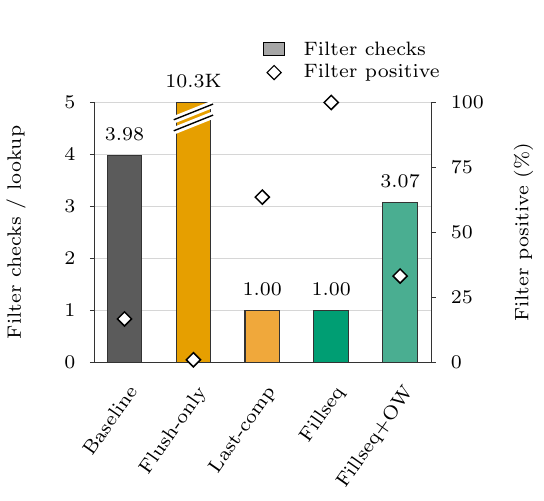
\begin{tikzpicture}[x=1cm,y=1cm,font=\small,
axis/.style={draw=black!80,line width=0.5pt},
grid/.style={draw=black!16,line width=0.4pt}]
\path[use as bounding box] (0,0) rectangle (6.200,5.650);
\draw[grid] (0.85,1.4000) -- (5.1300,1.4000);
\draw[axis] (0.79,1.4000) -- (0.85,1.4000);
\node[font=\fontsize{7}{8}\selectfont,anchor=east] at (0.7300,1.4000) {0};
\draw[grid] (0.85,2.0600) -- (5.1300,2.0600);
\draw[axis] (0.79,2.0600) -- (0.85,2.0600);
\node[font=\fontsize{7}{8}\selectfont,anchor=east] at (0.7300,2.0600) {1};
\draw[grid] (0.85,2.7200) -- (5.1300,2.7200);
\draw[axis] (0.79,2.7200) -- (0.85,2.7200);
\node[font=\fontsize{7}{8}\selectfont,anchor=east] at (0.7300,2.7200) {2};
\draw[grid] (0.85,3.3800) -- (5.1300,3.3800);
\draw[axis] (0.79,3.3800) -- (0.85,3.3800);
\node[font=\fontsize{7}{8}\selectfont,anchor=east] at (0.7300,3.3800) {3};
\draw[grid] (0.85,4.0400) -- (5.1300,4.0400);
\draw[axis] (0.79,4.0400) -- (0.85,4.0400);
\node[font=\fontsize{7}{8}\selectfont,anchor=east] at (0.7300,4.0400) {4};
\draw[grid] (0.85,4.7000) -- (5.1300,4.7000);
\draw[axis] (0.79,4.7000) -- (0.85,4.7000);
\node[font=\fontsize{7}{8}\selectfont,anchor=east] at (0.7300,4.7000) {5};
\draw[axis] (0.85,1.4000) -- (5.1300,1.4000);
\draw[axis] (0.85,1.4000) -- (0.85,4.7000);
\node[font=\fontsize{7}{8}\selectfont,rotate=90,anchor=south] at (0.1000,3.0500) {Filter checks / lookup};
\draw[axis] (5.13,1.4000) -- (5.13,4.7000);
\draw[axis] (5.13,1.4000) -- (5.19,1.4000);
\node[font=\fontsize{7}{8}\selectfont,anchor=west] at (5.2500,1.4000) {0};
\draw[axis] (5.13,2.2250) -- (5.19,2.2250);
\node[font=\fontsize{7}{8}\selectfont,anchor=west] at (5.2500,2.2250) {25};
\draw[axis] (5.13,3.0500) -- (5.19,3.0500);
\node[font=\fontsize{7}{8}\selectfont,anchor=west] at (5.2500,3.0500) {50};
\draw[axis] (5.13,3.8750) -- (5.19,3.8750);
\node[font=\fontsize{7}{8}\selectfont,anchor=west] at (5.2500,3.8750) {75};
\draw[axis] (5.13,4.7000) -- (5.19,4.7000);
\node[font=\fontsize{7}{8}\selectfont,anchor=west] at (5.2500,4.7000) {100};
\node[font=\fontsize{7}{8}\selectfont,rotate=90,anchor=north] at (6.0500,3.0500) {Filter positive (\%)};
% baseline: checks=3.982686247, positives=0.664776294, filter_positive_percent=16.691656154
\draw[draw=black!80,line width=0.4pt,fill=vb0] (1.01000,1.40000) rectangle (1.45000,4.02857);
\draw[draw=black,fill=white,line width=0.55pt] (1.2300,2.0408) -- (1.3200,1.9508) -- (1.2300,1.8608) -- (1.1400,1.9508) -- cycle;
\node[font=\fontsize{7}{8}\selectfont,anchor=south] at (1.2300,4.0986) {3.98};
\node[font=\fontsize{7}{8}\selectfont,rotate=55,anchor=north east] at (1.2300,1.3000) {Baseline};
% flush_only: checks=10254.443461744, positives=99.771162613, filter_positive_percent=0.972955412
\draw[draw=black!80,line width=0.4pt,fill=vb1] (1.88500,1.40000) rectangle (2.32500,4.70000);
\draw[draw=black,fill=white,line width=0.55pt] (2.1050,1.5221) -- (2.1950,1.4321) -- (2.1050,1.3421) -- (2.0150,1.4321) -- cycle;
\node[font=\fontsize{7}{8}\selectfont,anchor=south] at (2.1050,4.7700) {10.3K};
\draw[white,line width=2.6pt] (1.8550,4.3400) -- (2.3550,4.5400);
\draw[black,line width=0.5pt] (1.8550,4.3400) -- (2.3550,4.5400);
\draw[white,line width=2.6pt] (1.8550,4.4800) -- (2.3550,4.6800);
\draw[black,line width=0.5pt] (1.8550,4.4800) -- (2.3550,4.6800);
\node[font=\fontsize{7}{8}\selectfont,rotate=55,anchor=north east] at (2.1050,1.3000) {Flush-only};
% last_comp: checks=0.999994295, positives=0.635696105, filter_positive_percent=63.569973157
\draw[draw=black!80,line width=0.4pt,fill=vb2] (2.76000,1.40000) rectangle (3.20000,2.06000);
\draw[draw=black,fill=white,line width=0.55pt] (2.9800,3.5878) -- (3.0700,3.4978) -- (2.9800,3.4078) -- (2.8900,3.4978) -- cycle;
\node[font=\fontsize{7}{8}\selectfont,anchor=south] at (2.9800,2.1300) {1.00};
\node[font=\fontsize{7}{8}\selectfont,rotate=55,anchor=north east] at (2.9800,1.3000) {Last-comp};
% fillseq: checks=1.000000000, positives=1.000000000, filter_positive_percent=100.000000000
\draw[draw=black!80,line width=0.4pt,fill=vb3] (3.63500,1.40000) rectangle (4.07500,2.06000);
\draw[draw=black,fill=white,line width=0.55pt] (3.8550,4.7900) -- (3.9450,4.7000) -- (3.8550,4.6100) -- (3.7650,4.7000) -- cycle;
\node[font=\fontsize{7}{8}\selectfont,anchor=south] at (3.8550,2.1300) {1.00};
\node[font=\fontsize{7}{8}\selectfont,rotate=55,anchor=north east] at (3.8550,1.3000) {Fillseq};
% fillseq_ow: checks=3.070917812, positives=1.019486067, filter_positive_percent=33.198090266
\draw[draw=black!80,line width=0.4pt,fill=vb4] (4.51000,1.40000) rectangle (4.95000,3.42681);
\draw[draw=black,fill=white,line width=0.55pt] (4.7300,2.5855) -- (4.8200,2.4955) -- (4.7300,2.4055) -- (4.6400,2.4955) -- cycle;
\node[font=\fontsize{7}{8}\selectfont,anchor=south] at (4.7300,3.4968) {3.07};
\node[font=\fontsize{7}{8}\selectfont,rotate=55,anchor=north east] at (4.7300,1.3000) {Fillseq+OW};
\draw[draw=black,fill=black!35] (3.00,5.30) rectangle (3.26,5.46);
\node[font=\fontsize{7}{8}\selectfont,anchor=west] at (3.3800,5.3800) {Filter checks};
\draw[draw=black,fill=white] (3.13,5.17) -- (3.22,5.08) -- (3.13,4.99) -- (3.04,5.08) -- cycle;
\node[font=\fontsize{7}{8}\selectfont,anchor=west] at (3.3800,5.0800) {Filter positive};
\end{tikzpicture}
\endgroup
